%%%%%%%%%%%%%%%%%%%%%%%%%%%%%%%%%%%%%%%%%%%%%%%%
%%%%%%%%%%%%%%%%%%%%%%%%%%%%%%%%%%%%%%%%%%%%%%%%
\begin{frame}
  \frametitle{(Pre-)Exascale machines - architecture diversity !}

  \begin{itemize}
  \item \textcolor{red}{\bf \large US}: Summit , Sierra $\Rightarrow$ mostly OpenPower (IBM P9 + Nvidia V100), GPU-based architecture, \#2 and \#3 @top500; exascale machines announced
    \begin{itemize}
     \item \myhref{https://www.nextplatform.com/2019/03/18/intel-to-take-on-openpower-for-exascale-dominance-with-aurora/}{Aurora} (Argonne NL, 2022): Intel \myhref{https://www.nextplatform.com/2018/12/16/intel-unfolds-roadmaps-for-future-cpus-and-gpus/}{Xe GPU}
     \item \myhref{https://www.nextplatform.com/2019/05/07/cray-amd-tag-team-on-1-5-exaflops-frontier-supercomputer/}{Frontier} (Oak Ridge NL, 2021 ?): AMD EPYC + Radeon Instinct GPU
    \end{itemize}
  \item \textcolor{blue}{\bf \large China:}
    \begin{itemize}
    \item Phytium FT2000/64 ARM chips + Matrix2000 GPDSP accelerators $\Rightarrow$ \#6 @top500, Tianhe-2A, 61 PFlops
    \item 260-core Shenwei, \textcolor{blue}{\bf homegrow technology} hardware + software (C++/fortran compiler + OpenACC) $\Rightarrow$ \#4 @top500 , Sunway TaihuLight, 105 PFlops
    \item Dhyana, AMD-licenced x86 multicore (300 M\$), identical to AMD EPYC
      % https://www.top500.org/news/china-reveals-third-exascale-prototype/
    \end{itemize}

  \item \textcolor{violet}{\bf \large Japan:} \myhref{https://postk-web.r-ccs.riken.jp/spec.html}{\bf Fugaku}(Fujitsu, ARM, RIKEN)  A64FX ARM (\textcolor{violet}{\bf home grown}, started in 2014, \textcolor{violet}{\bf \#1 @top500 (Nov. 2020)}, 900 M\$), GPU, etc ...
    % https://www.hpcwire.com/2018/09/05/no-go-for-glofo-at-7nm-and-the-fujitsu-a64fx-post-k-cpu/
    % https://www.top500.org/news/fujitsu-reveals-details-of-processor-that-will-power-post-k-supercomputer/
    % http://www.fujitsu.com/jp/Images/20180821hotchips30.pdf
    % https://www.theregister.co.uk/2018/08/22/fujitsu_post_k_a64fx/
  \item \textcolor{darkgreen}{\bf \large Europe} : new organization EuroHPC (2018), EC H2020 budget ($\sim$ 500 M\euro{} per year)\\
    \textcolor{darkgreen}{\bf home grown} (EPI) ARM and RISC-V architecture, early stage%just starting development
    % https://www.top500.org/news/european-program-to-develop-supercomputing-chips-begins-to-take-shape/
    % mettre une EPI roadmap
    % EuroHPC (Nov. 2018 - 2026)
    % EuroHPC, Exascale not before 2022 : https://www.youtube.com/watch?v=y7_VvcIKJnI
    % EuroHPC 2 exascale machines (500 M€)
    % EuroHPC 2 pre-exascale machines in 2021 (240 M€)
  \end{itemize}

  %{\tiny \myurl{https://www.nextplatform.com/2016/07/11/chinas-triple-play-pre-exascale-systems/}}

\end{frame}

%%%%%%%%%%%%%%%%%%%%%%%%%%%%%%%%%%%
%%%%%%%%%%%%%%%%%%%%%%%%%%%%%%%%%%%
\begin{frame}
  \frametitle{Motivations for performance portability}

  \begin{itemize}
  \item {\Large What is performance portability ?}
    \begin{itemize}
    \item \textcolor{violet}{\large \bf (Re)write your code once, (try to) run {\it efficiently} everywhere}
    \item By everywhere, we mean : Multicore Intel/ARM and Nvidia/AMD GPUs
    \item \textcolor{violet}{\bf High-level approach:} as much as possible (if possible) hide hardware details to the (physicist / applied math) software developer
    \item \myhref{https://performanceportability.org}{https://performanceportability.org}
    \item \myhref{https://asc.llnl.gov/doe-coe-mtg-2016}{1st annual DOE Performance Portability Meeting (2016)}
    \end{itemize}
  \item {\large Is that \textcolor{darkgreen}{\bf possible} ? How ? Which programming model ? Which language ? Which compiler ? $\Rightarrow$ large combinatorics}
  \item for the rest of this talk, i'll focus on the \myhref{https://github.com/kokkos/kokkos}{kokkos/C++} library
  \end{itemize}

\end{frame}

%%%%%%%%%%%%%%%%%%%%%%%%%%%%%%%%%%%%%%%%%%%%%%%%
%%%%%%%%%%%%%%%%%%%%%%%%%%%%%%%%%%%%%%%%%%%%%%%%
\begin{frame}
  \frametitle{Parallel programming models landscape}

  \begin{minipage}{0.73\linewidth}
    \begin{itemize}
    \item \textcolor{red}{\textbf{Low-level native language:}} \myhref{https://www.khronos.org/opencl/}{OpenCL}, \myhref{https://developer.nvidia.com/cuda-downloads}{CUDA}, \myhref{https://rocmdocs.amd.com/en/latest/Programming_Guides/Programming-Guides.html}{HIP}
    \item \textcolor{orange}{\textbf{Directive approach (code annotations)}} for multicore/GPU, ...:
      \begin{itemize}
      \item \myhref{http://www.openmp.org/}{OpenMP} 5.1 (Clang, PGI, GNU, ...), \myhref{https://pm.bsc.es/ompss-2}{OmpSs-2}
      \item \myhref{http://www.openacc.org/}{OpenACC} 2.7 (PGI, GNU, ...) \textcolor{blue}{$\Rightarrow$ Fortran codes.}
      \end{itemize}
    \item \textcolor{darkgreen}{\textbf{Other high-level library-based approaches}}:
      {
        \scriptsize
        \begin{itemize}
        \item \framebox{\myhref{https://github.com/kokkos/kokkos}{Kokkos}}, \myhref{https://github.com/LLNL/RAJA}{RAJA}, \myhref{https://github.com/alpaka-group/alpaka}{Alpaka}, \myhref{https://github.com/STEllAR-GROUP/hpx}{HPX}, \myhref{https://github.com/GridTools/gridtools}{GridTools}, \myhref{https://arrayfire.com/}{ArrayFire}...
        \item \myhref{https://www.khronos.org/sycl}{SYCL} (Khronos Group \textit{standard}), C++ high-level layer on top of OpenCL. %\textcolor{red}{\bf Still $\sim$experimental}\\
          \myhref{https://software.intel.com/content/www/us/en/develop/tools/oneapi.html}{Intel OneAPI/DPCPP} (Intel CPU/GPU/FPGA, Nvidia GPUs),\\
          \myhref{https://www.codeplay.com/products/computesuite/computecpp}{CodePlay},
          \myhref{https://github.com/illuhad/hipSYCL}{AMD and Nvidia GPUs},
          \myhref{https://github.com/keryell/triSYCL}{Keryell/Xilinx}
        \item {\bf C++-17 built-in parallelism for multicore and GPUs}, e.g.:
          \begin{itemize}
          \item Nvidia's \myhref{https://developer.nvidia.com/hpc-sdk}{hpc-sdk} (May 2020)
          \item \myhref{https://github.com/oneapi-src/oneTBB}{Intel OneAPI/TBB}
          \end{itemize}
        \end{itemize}
      }
    \end{itemize}
  \end{minipage}
  %
  \begin{minipage}{0.26\linewidth}
    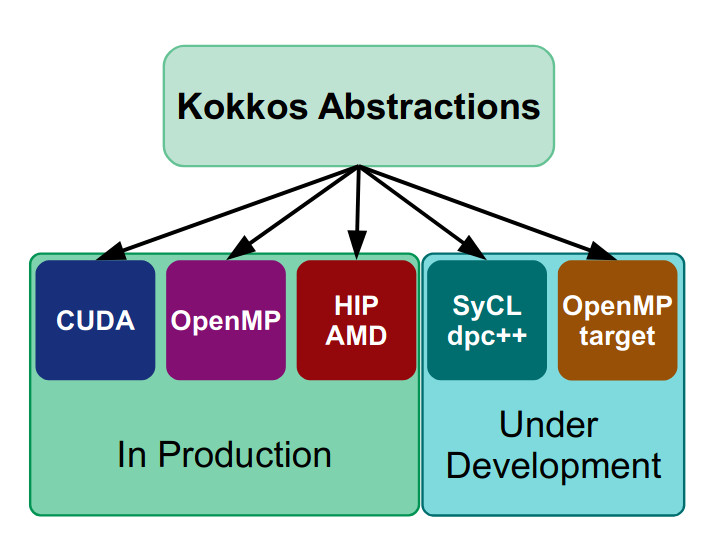
\includegraphics[width=1.3\linewidth]{./images/exascale/kokkos_backends}

    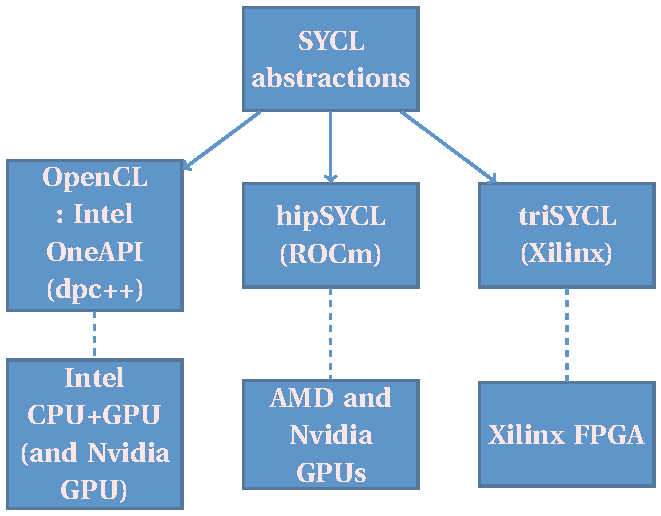
\includegraphics[width=1.3\linewidth]{./tikz/sycl}

    %\textcolor{blue}{\bf \scriptsize All these programming solutions are interconnected and inter-dependent !}

    {
      \scriptsize
      {\bf additionnal features:}\\
      \textcolor{violet}{\bf memory management,}\\
      \textcolor{violet}{\bf data containers}, ...
    }

  \end{minipage}

\end{frame}

%%%%%%%%%%%%%%%%%%%%%%%%%%%%%%%%%%%%%%%%%%%%%%%%%%%%%%%%%%%%%%%%%%%
%%%%%%%%%%%%%%%%%%%%%%%%%%%%%%%%%%%%%%%%%%%%%%%%%%%%%%%%%%%%%%%%%%%
%%%%%%%%%%%%%%%%%%%%%%%%%%%%%%%%%%%%%%%%%%%%%%%%%%%%%%%%%%%%%%%%%%%
\begin{frame}
  \frametitle{Kokkos: a programming model for perf. portability}

  \only<1>{
    \begin{itemize}
    \item \textcolor{blue}{\textbf{Kokkos}} is a \textbf{C++ library} for \textcolor{violet}{\textbf{node-level parallelism}} (i.e. \textcolor{violet}{\bf shared memory}) providing abstractions for {\bf harware-aware}:

      \begin{itemize}
      \item \textcolor{red}{\textbf{parallel algorithmic patterns}}
      \item \textcolor{red}{\textbf{data containers}}
      \end{itemize}
    \item \myurl{https://kokkos.org/}
    \item Implementation relies heavily on \textbf{C++ meta-programing} to derive native low-level code (OpenMP, CUDA, HIP, SYCL...) and adapt data structure memory layout at compile-time
    \item Developped at \textcolor{violet}{\textbf{Sandia NL}} (core, CUDA, OpenMP), \textcolor{violet}{\textbf{ORNL}} (HIP, SYCL), ...
    \end{itemize}

    \textcolor{darkgreen}{\bf Goal:} {\bf write one implementation which:}
    \begin{itemize}
    \item compiles and \textcolor{blue}{\bf run on multiple archs},
    \item obtains \textcolor{blue}{\bf performant memory access pattern} across archs,
    \item can leverage \textcolor{blue}{\bf arch-specific features} where possible.
    \end{itemize}

  }
  \only<2>{
    \begin{itemize}
    \item \textcolor{darkgreen}{\textbf{Open source}}, \myurl{https://github.com/kokkos/kokkos}, since $\sim 2012$
    \item Primarily developped as a base building layer for \textbf{generic high-performance parallel linear algebra} in \myhref{https://github.com/trilinos/Trilinos}{Trilinos}
    \item Used in, e.g.:
      \begin{itemize}
      \item \myhref{http://lammps.sandia.gov/}{LAMMPS} (molecular dynamics code),
        %\myhref{https://github.com/ECP-copa/ExaMiniMD}{ExaMiniMD}
      \item \myhref{https://github.com/NaluCFD/Nalu}{NALU CFD} (low-Mach wind flow),
      \item \myhref{https://sparta.sandia.gov/}{SPARTA/DSMC} (rarefied gas flow), \myhref{}{SPARC} (CFD, RANS, LES, hypersonic flow)
      \item \myhref{https://github.com/SNLComputation/Albany}{Albany} (fluid/solid,...)
      \item \myhref{http://uintah.utah.edu/}{Uintah} (structured AMR, combustion, radiation)
        % \item list of codes using Kokkos: \myurl{https://github.com/kokkos/kokkos/issues/1950}
      %\item \myhref{https://github.com/kokkos/kokkos/issues/1950}{list of codes using Kokkos}
      \end{itemize}

      % \item Goal: \textcolor{orange}{\textbf{ISO/C++ 2020 Standard}} subsumes Kokkos abstractions~\footnote{\scriptsize see mdspan proposal \myurl{https://github.com/kokkos/array_ref}}
    \end{itemize}
  }

  \only<2>{
  \begin{columns}
    \begin{column}{0.34\linewidth}
      Strong involvement in \textcolor{orange}{\textbf{ISO/C++ 2020 Standard}}\\
      Make Kokkos a sliding window of future c++ features
    \end{column}
    \begin{column}{0.65\linewidth}
      \begin{center}
        \includegraphics<1-2>[width=5cm]{images/perf_portability/kokkos_summary}
      \end{center}
    \end{column}
  \end{columns}
  \vfill
  {
    \scriptsize see mdspan proposal \myurl{https://github.com/kokkos/mdspan}\\
    \myurl{https://arxiv.org/abs/2010.06474}
  }
}

\end{frame}

%%%%%%%%%%%%%%%%%%%%%%%%%%%%%%%%%%%%%%%%%%%%%%%%%%%%%%%%%%%%%%%%%%%
%%%%%%%%%%%%%%%%%%%%%%%%%%%%%%%%%%%%%%%%%%%%%%%%%%%%%%%%%%%%%%%%%%%
%%%%%%%%%%%%%%%%%%%%%%%%%%%%%%%%%%%%%%%%%%%%%%%%%%%%%%%%%%%%%%%%%%%
\begin{frame}
  \frametitle{Kokkos: a programming model for perf. portability}

  \begin{center}
    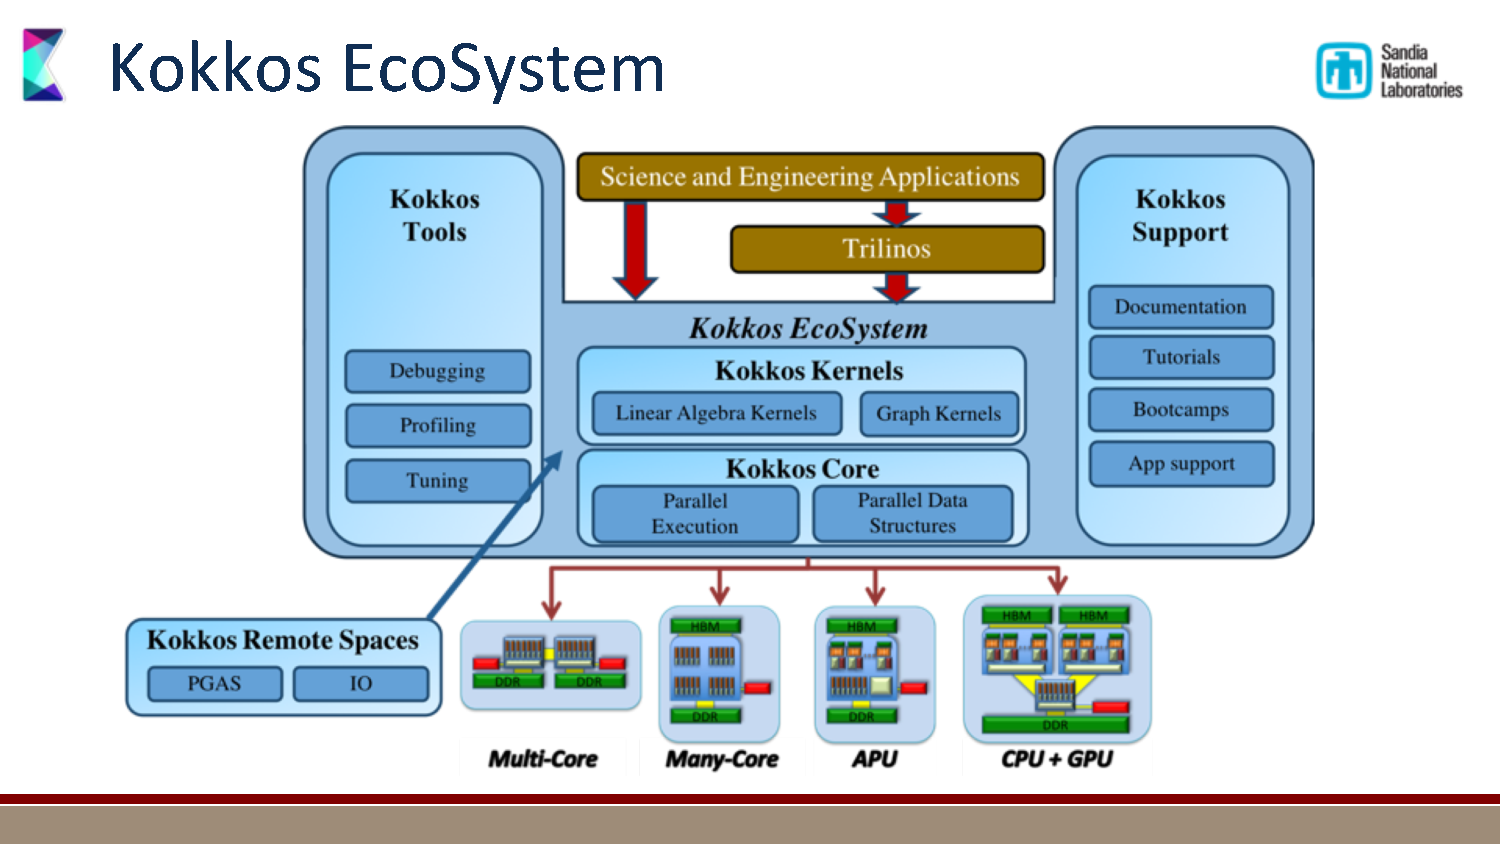
\includegraphics[width=0.8\linewidth]{images/kokkos/trott1}
  \end{center}

  { \tiny
    \begin{itemize}
    \item \myhref{https://github.com/kokkos/kokkos-kernels}{Kokkos-kernels} (many dense/sparse BLAS problems, ...)
    \item \myhref{https://github.com/kokkos/kokkos-fortran-interop}{Fortran compatibility layer} (REX code \myhref{https://ecpannualmeeting.com/assets/overview/sessions/XGC_ECP_2020.pptx}{XGC-Cabana}, Plasma physics, Gyrocinetics, particle-in-cell)
    \item interface python (\myhref{https://github.com/pybind/pybind11}{pybind11}-based)
    \item \myhref{https://prod-ng.sandia.gov/techlib-noauth/access-control.cgi/2017/1710464.pdf}{Task-DAG parallelism (CPU / GPU)}
    \end{itemize}
  }

  source: C. Trott, DOE Performance Portability Meeting, April 2019
\end{frame}

%%%%%%%%%%%%%%%%%%%%%%%%%%%%%%%%%%%
%%%%%%%%%%%%%%%%%%%%%%%%%%%%%%%%%%%
% \begin{frame}
%   \frametitle{C++ Kokkos library summary}

%   \begin{itemize}
%   %\item See GTC2017 session \textcolor{violet}{S7344 - Kokkos ? The C++ Performance Portability Programming Model} (C. Trott and H.C. Edwards).
%   \item Framework for efficient \textcolor{RedOrange}{\bf node-level parallelism (CPU, GPU, ...)}
%   \item Provides
%     \begin{itemize}
%     \item \textcolor{blue}{\bf Computationnal parallel patterns} (for, reduce, scan, ...)
%     \item \textcolor{violet}{\bf Hardware aware memory containers}: e.g. {\bf A multi-dimensionnal data container with hardware adapted memory layout}
%     \item Support for multiple backends:
%       {\scriptsize
%         \begin{itemize}
%         \item OpenMP (x86, ARM, IBM, ...)
%         \item pthreads
%         \item OpenMP target (GPU, ...),
%         \item CUDA (Nvidia GPU, ...),
%         \item HIP (AMD and Nvidia GPU),
%         \item SYCL (Intel CPU and GPU, Nvidia, ...)
%         \item HPX
%         \end{itemize}
%       }
%     \item Additionnal sub-projects: \myhref{https://github.com/kokkos/kokkos-kernels}{kokkos-kernels} (BLAS, sparse BLAS, Graph), \myhref{https://github.com/kokkos/simd-math}{Kokkos::simd}, \myhref{https://github.com/kokkos/kokkos-python}{python bindings}, ...

%     \end{itemize}
%   % \item Provides some {\bf \textcolor{RedOrange}{high-level (abstract) concepts}} as template C++ classes:
%   %   \begin{itemize}
%   %   \item A \textcolor{red}{\bf kokkos device:} \texttt{Kokkos::Cuda, Kokkos::OpenMP, Kokkos::Pthreads, Kokkos::Serial},...
%   %   \item concepts controlled by C++ template meta-programing: \textcolor{darkgreen}{\bf execution space, memory space, memory layout, ...}
%   %   \item \textcolor{blue}{\bf Computationnal parallel patterns} (for, reduce, scan, ...) controlled with a {\bf execution policy} (i.e. how many iterations, teams, ...)
%   %   \end{itemize}
%   % \item \textcolor{violet}{\bf \texttt{Kokkos::View}}: {\bf A multi-dimensionnal data container with hardware adapted memory layout} \\
%   %   % with ability to mirror view between memory spaces, ...
%   %   {\small
%   %     -\;\textcolor{violet}{\texttt{Kokkos::View<double **> data("data",NX,NY);}} // 2D array with sizes known at runtime\\
%   %     -\;\framebox{{\bf How do I access data ?} \texttt{data(i,j)} !}
%   %   }
%   \item Mostly a header library (C++ metaprogramming)
%   %\item build system / module load / etc ... (?)
%   \end{itemize}

% \end{frame}

%%%%%%%%%%%%%%%%%%%%%%%%%%%%%%%%%%%
%%%%%%%%%%%%%%%%%%%%%%%%%%%%%%%%%%%
% \begin{frame}
%   \frametitle{C++ Kokkos library summary}

%   % I started using Kokkos in June 2016, shortly developped 2D Hydro MUSCL-Hancok 2nd order scheme.

%   \begin{itemize}
%   \item {\bf What does it mean hardware aware memory containers ?}
%   \item Most commonly in a C/C++, {\bf multi-dimensionnal array access} is done through {\bf \textcolor{red}{index linearization}} (row or column-major in 2D):
%     $$ \mathbf{index} = \mathbf{i} + nx * \mathbf{j}  + nx*ny * \mathbf{k}$$
%   \item {\bf Fortran} (column-major format) vs {\bf C/C++} (row-major format)
%   \item There is no reason to favour one layout versus the other
%     \begin{itemize}
%     \item column-major is better for vectorization on CPU architecture
%     \item row-major is better for high througput architecture e.g. GPU (memory coalescence)
%     \item $\Rightarrow$ \textcolor{orange}{\bf Kokkos allows to chose memory layout at compile time}
%     \end{itemize}
%   \item In Kokkos, one should/must avoid this index linearization at the user level, let \texttt{Kokkos::View} do this job (\textcolor{darkgreen}{\bf decided at compile-time, hardware adapted})
%     $$ \text{data}(i,j,k) $$
%     % \begin{itemize}
%     % \item 1D \texttt{Kokkos::View} with user-defined index linearization + 1D Iteration range
%     % \item \textcolor{blue}{2D \texttt{Kokkos::View}  + 1D flat Iteration range} {\bf (used in this work)}
%     % \item 2D \texttt{Kokkos::View}  + 2D (\texttt{Kokkos::MDRange} Kernel policy) : still an experimental feature
%     % \end{itemize}
%   %\item \texttt{Kokkos::MDRange} is functional, but was generating kernels with some performance loss, will surely be solved shortly by Kokkos core developpers.
%   %\item See also new developpement on hierarchical task-data parallelism, session S7253 (Monday 8th, room 211B).
%   \end{itemize}

%   % Some personnal views / experience as an external Kokkos user

% \note[item]{Let me brievely add a comment on memory layout, which is an important feature. With kokkos, array linearization is a low-level implementation detail, that must be abstracted away, if I may say. This way, the end-programmer only access data using a multi-index set, linearization is done in an hardware-aware way by kokkos at compile time, once the target device has been specified.}

% \end{frame}

